\documentclass[12pt]{article}

\usepackage[english]{babel}
\usepackage[utf8x]{inputenc}
\usepackage{pdfpages}
\usepackage{lastpage} % Required to determine the last page for the footer
\usepackage{extramarks} % Required for headers and footers
\usepackage{graphicx} % Required to insert images
\usepackage{listings} % Required for insertion of code
\usepackage{courier} % Required for the courier font
\usepackage{color}
\usepackage{grffile}
\usepackage{float}

\usepackage[a4paper, total={6in, 8in}]{geometry}

% Margins
\topmargin=-0.45in
\evensidemargin=0in
\oddsidemargin=0in
\textwidth=6.5in
\textheight=9.0in
\headsep=0.25in
\fboxsep=0mm%padding thickness
\fboxrule=2pt%border thickness

\linespread{1.1} % Line spacing

\newcommand{\Title}{Functional requirements and application design document} % Assignment title
\newcommand{\Class}{Cos\ 301} % Course/class
\newcommand{\pd}{Post-Doctoral}
\newcommand{\ssr}{Soft\color{green}{Serve }\color{black}}
\newcommand{\version}{0.9}
\newcommand{\iteration}{1}
\newcommand{\client}{Ms. Cathy Sandis (UP Research Office)}
\newcommand{\project}{Post-Doctoral Application Management System}

\begin{document}


\vspace{4em}

\begin{center}%

\begin{figure}[ht!]
\centering

\includegraphics{../Images_Docs/logo.png}
\end{figure}
\LARGE \bf \project \\[1em]
\LARGE \bf \Title \\[0.25em]
\large \bf \today\\
\bf Version \version\\
\bf Iteration \iteration\\[0.5em]
\Large \bf Prepared for \client\\
\Large \bf by
\Large {\bf \ssr Group }\\[0.5em]
\LARGE {\bf Group members}\\[0.25em]
\large
Kgothatso Phatedi Alfred Ngako (12236731) \\[0.5em]
Tokologo “Carlo” Machaba (12078027) \\[0.5em]
Mathys Ellis (12019837) \\[8em]

\end{center}%

%\newpage
%{\LARGE \bf Change log}\\[2em]

\begin{center}
\begin{tabular}{|l|p{1.4cm}|p{8cm}|p{2.8cm}|}
\hline
\multicolumn{4}{|c|}{\bf Change log} \\
\hline
 Date & Version & Description &  Person \\
\hline
10/02/2014 & v 0.0 & Original SRS document created & Mathys Ellis \\
\hline
02/03/2014 & v 0.1 & Added to glossary & Mathys Ellis \\
\hline
11/03/2014 & v 0.2 & Added more functional requirements which relate more to the use case diagrams & Alfred Ngako \\
\hline
16/03/2014 & v 0.3 & Added domain objects data relation diagrams & Alfred Ngako \\
\hline
16/03/2014 & v 0.4 & Added some preconditions and did some formatting & Mathys Ellis \\
\hline
17/03/2014 & v 0.5 & Added rest of preconditions and all the postconditions. Also added to the glossary & Mathys Ellis \\
\hline
20/03/2014 & v 0.6 & Updated the domain objects diagram  & Mathys Ellis \\
\hline
20/03/2014 & v 0.65 & Updated the domain objects plus diagram  & Alfred Ngako \\
\hline
20/03/2014 & v 0.7 & Updated the use case prioritization  & Alfred Ngako \\
\hline
16/03/2014 & v 0.75 & Did some restructuring and document formatting & Mathys Ellis \\
\hline
17/03/2014 & v 0.8 & Added to the glossary & Mathys Ellis \\
\hline
12/05/2014 & v 0.9 & Created new Functional requirements and application design document. & Mathys Ellis \\
\hline
15/05/2014 & v 0.91 & Transferred necessary content from old SRS document. Performed editing and restructuring of document. & Mathys Ellis \\
\hline
15/05/2014 & v 0.92 & Added and redefined domain objects. & Mathys Ellis \\
\hline

%\end{tabbing}
\end{tabular}
\end{center}
\newpage
\tableofcontents

\listoffigures
\newpage
\section{Document description:}

\subsection{Document purpose:}
\vspace{0.2in}
This functional requirements and application design document serves the purpose of providing a detailed breakdown of the SoftServe's Post-Doctoral application management system's expected functionality and how it will be realised in terms of application design. Further it defines the services contracts required by each of the stakeholders with the proposed software system. Thus this document serves as a contract between SoftServe and the client, Mrs Cathy Sandis of the DRIS of the University of Pretoria in terms of project functional requirements.

\vspace{0.2in}

\subsection{Documentation methodology}
\vspace{0.2in}
\begin{flushleft}
The documentation and software development methodology used by the project adhere to the guidelines set out by the agile method. Thus this document has undergone and will undergo various iterations that may extend or reduce the contents of the document.\\

This document was created using the requirement elicitation techniques and requirement definitions as specified by Klaus Pohl’s book Requirements Engineering: Fundamentals, Principles, and Techniques [Dr.Phol, K., 2010].
The requirements, vision and scope were elicited from the following sources:
\begin{itemize}
	\item Numerous interviews with the client.
	\item On-line research into UP Post doctoral applications.
	\item Correspondence with the UP IT department.
	\item Collecting and analysing various documents such as:
		\begin{itemize}
			\item The initial project request document
			\item Application forms
			\item Renewal forms
			\item CV templates
			\item Approval and recommendation forms
		\end{itemize}
\end{itemize}
\end{flushleft}	

\vspace{0.5in}

\subsection{Document conventions:}
\vspace{0.1in}
\begin{itemize}
\item Documentation formulation tool: LaTeX
\item ERD Crow-Foot notation
\item UML 2.0
\end{itemize}

\vspace{0.2in}

\subsection{References:}
\vspace{0.1in}
\begin{itemize}
\item Dr.Phol, K., 2010, \textit{Requirements Engineering: Fundamentals, Principles, and Techniques}, Springer, Heidelberg.
\end{itemize}	

\vspace{0.5in}

\newpage
\section{Functional requirements}
\subsection{Introduction} %Alfred
\vspace{0.2in}
This section discusses the functional requirements for SoftServe's Post-Doctoral application management system.
The required functionality, domain objects, process specification and use cases related to the functional requirements of the project will be discussed.
\vspace{0.2in}

\subsection{Required functionality} %Alfred
\vspace{0.2in}
The following sections will discuss the required functionality of all the major services handled by the system. Namely:
\begin{itemize}
\item Application service
\item Report services
\item Notification services
\item User account management services
\item Audit-Trail services
\item Archival services
\end{itemize}

%Use the use case diagrams to complete the requirements of each of the services in the format I provided
\subsubsection{Application services}
		The application services encompasses the the entirety of the of the application process undergone by prospective fellows namely new and renewal applications.
		The main user of these services will be the prospective fellows who wishes to track their application progress or renew or apply for a Post-Doctoral fellowship. Other stakeholders will only make use of certain sub-services which are provided under the Application services. It should be noted that most of the different stakeholders' usage will be focused in this set of services only.
		
		\begin{itemize}
			\item New fellowship application service API:		
			\begin{enumerate}
				\item Account creation for new prospective fellows, referees and grant holders.
				\item All internal stakeholders should be able to log in with their PeopleSoft account details when the system is integrated but until such time they will be provided with account creation options.				
				\item A prospective fellow should be able to open a new application.
				\item A prospective fellow should be able to add their CV in the required format.
				\item A specified grant holder should be able to add their CV in the required format.
				\item A owner of a CV should be able to add various qualifications and work experience to their CV.
				\item A owner of a CV should be able to update their CV if it has been created. 
				\item A prospective fellow should be able to specify their intended grant holder.	
				\item A prospective fellow should be able to specify their intended referees.
				\item A specified grant holder should be able to complete the prospective fellows application.
				\item A application should be made available for stakeholders such as the DRIS, HOD and Dean to deny or approve it at the correct stage in the process.
				\item A referee should be able to login and create a referral report for the prospective fellow that identified him/her.
				\item A HOD of a department should be able to login and approve, decline or ask for amendment of any pending applications.
				\item A HOD of a department must be able to create a recommendation report for applications they approve.
				\item A member of the dean's office should be able to login and endorse the applications that they approve with a motivation and be able to rank them.
				\item A DRIS member who administers the process must be able to log in and review pending applications that need to be checked for eligibility and approve or deny them.
				\item A DRIS member who administers the process must be able to create post doctoral committee meetings. And also be able to create the prepare the document their of.
				\item A DRIS member who administers the process must be able to finally approve or deny the funding of any last stage applications and also be able to provide motivation thereof.
				\item A member of the Post-Doctoral committee must be able to create minutes for a active meeting. 		
			\end{enumerate}
			
			\item Fellowship renewal service API:
			\begin{enumerate}		
				\item All internal stakeholders should be able to log in with their PeopleSoft account details once the system is integrated but until such time they should login with the credentials specified at the time of account creation.	
				\item A prospective fellow should be able to open a new renewal application. 
				\item A prospective fellow should be able to add their progress report on all the work they have been working on. 
				\item A prospective fellow's grant holder should be able to finalise the renewal application.
				\item The renewal application should be made available to the DRIS, HOD and dean to deny or approve it at the correct stage in the process.
				\item A HOD of a department should be able to login and approve, decline or ask for amendment of any pending applications.
				\item A HOD of a department must be able to create a recommendation report for applications they approve.
				\item A member of the dean's office should be able to login and endorse the applications that they approve with a motivation and be able to rank them.
				\item A DRIS member who administers the process must be able to log in and review pending applications that need to be checked for eligibility and approve or deny them.
				\item A DRIS member who administers the process must be able to create post doctoral committee meetings. And also be able to create the prepare the document their of.
				\item A DRIS member who administers the process must be able to finally approve or deny the funding of any last stage applications and also be able to provide motivation thereof.
				\item A member of the Post-Doctoral committee must be able to create minutes for a active meeting. 					
			\end{enumerate}
			\item Application progress viewer service API:
			\begin{enumerate}
				\item A prospective fellow should be able to login with their user account details.
				\item A prospective fellow's application status should be made available for their review if they have an application in the system.			
			\end{enumerate}
		\end{itemize}

\subsubsection{Report services}
The report services provides the reporting generation service for the DRIS in order to extract valuable information and allow them to provide electronic and hard copy data for review or archiving. The DRIS is the only stakeholder that will make use of this system. Note a reports are temporal objects and do not get saved by the system.
\begin{itemize}
	\item A DRIS member must be able to into the system and get access to the reporting module.
	\item The DRIS member must be able to access a report generation tool which effectively allows them to:
	\begin{enumerate}
		\item Open new report.
		\item Select report data from the database.
		\item Generate report.
		\item View report.
	\end{enumerate}
	\item The DRIS member viewing the report must be allowed to be exported the report to either a pdf or a spreadsheet format.
	
\end{itemize}
\subsubsection{User account management services} %Couldn't see who the actor is on the use case diagram
The user account management services provide each user who has an account on the system with the facilities to manage their account and also a facility for the system administrator to manage the accounts on the system.
\begin{itemize}
	\item Allow users to login.
	\item A prospective fellow will be create a new account if they don't have one.
	\item Any identified grant holder or referee that is not already on the system should be allowed to create a new account.
	\item If integrated with peoplesoft the system should be able to pull all the account information of personnel but until such time the system administrator will have to be allowed create the accounts of all DRIS members, Dean's office members, HODs and post-doctoral committee members.	
	\item A user should be able to modify their account details.
	\item A administrator should be able to modify any user account details.
	\item A administrator should be able to remove any user account.
\end{itemize}
\subsubsection{Notification services}
The system will need to generate automated notifications that are sent internally and to the corresponding email of the recipient. This service should also be provided to users with in the system with the correct privileges.
\begin{itemize}
	\item Stakeholders must be able to create a new notification.
	\item A notification must have recipient.
	\item A notification must have a non-empty message.
	\item A notification must be sent to both the user account and recipient's email address.
\end{itemize}

\subsubsection{Audit-Trail services}
The Audit-Trail services provide a means for the system administrator or DRIS members to view all the actions that were performed by a user of the system. It is important to note that the audit entries is read-only and can only be updated by the system itself. The monitored actions are hard wired into the system so to prevent any tampering.
\begin{itemize}
	\item An authorised user must be able to generate a report via the reporting services for the audit log.
	\item The system should be able to insert audit log entries when the monitored actions occur.
\end{itemize}
\subsubsection{Archival services}
The archival services of the system will be able to back up the current state of the database to a specified location. Further it should be able to remove old records from the working database that are no longer in use and store then in a location so that they can be retrieved on a on-demand basis.
\begin{itemize}
	\item The system administrator needs to be able to perform a automatic archival of old data.
	\item The system should be able to notify the system administrator of any possible archival data.
\end{itemize}
\vspace{0.2in}

\subsection{Use case diagrams}
\begin{figure}[H]
\centering	
\framebox{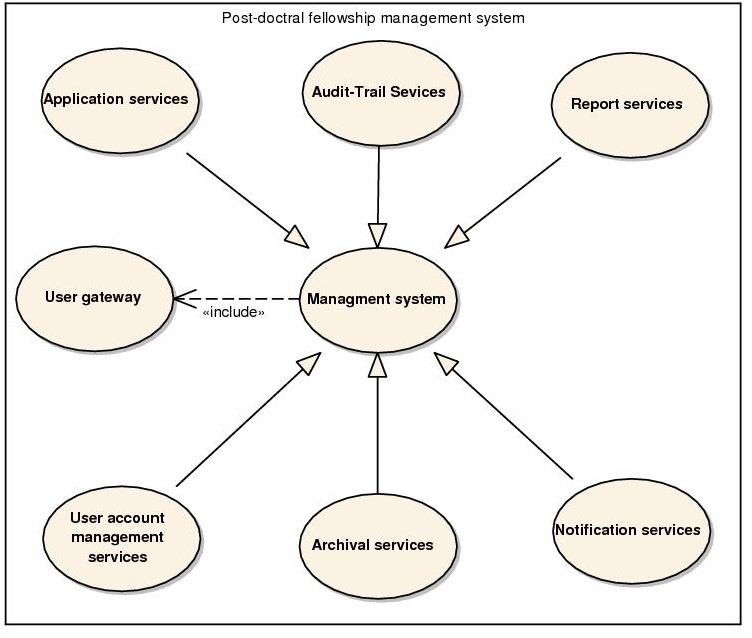
\includegraphics[scale=0.6]{../Images_Docs/Diagrams/Post-doctral fellowship management system.jpg}}
\caption{Use case diagram of Post-doctoral fellowship management system}
\end{figure}

\begin{figure}[H]
\centering	
\framebox{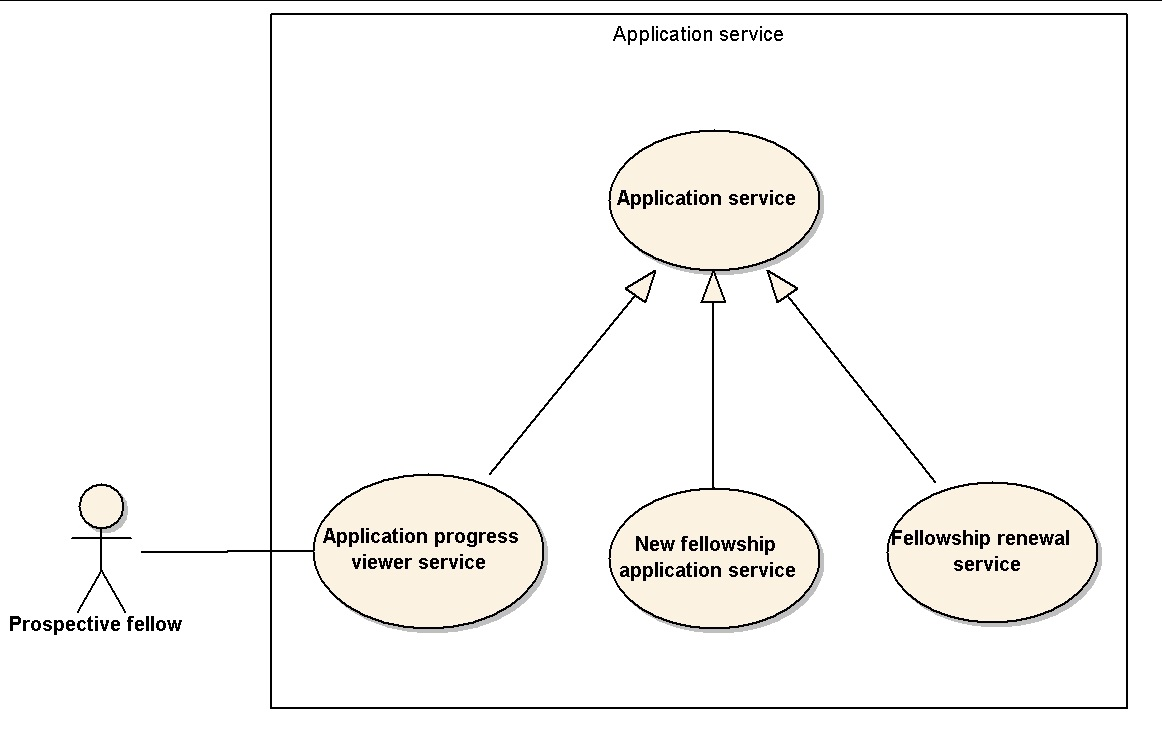
\includegraphics[scale=0.6]{../Images_Docs/Diagrams/Application service.jpg}}
\caption{Use case diagram of Application service}
\end{figure}

\begin{figure}[H]
\centering	
\framebox{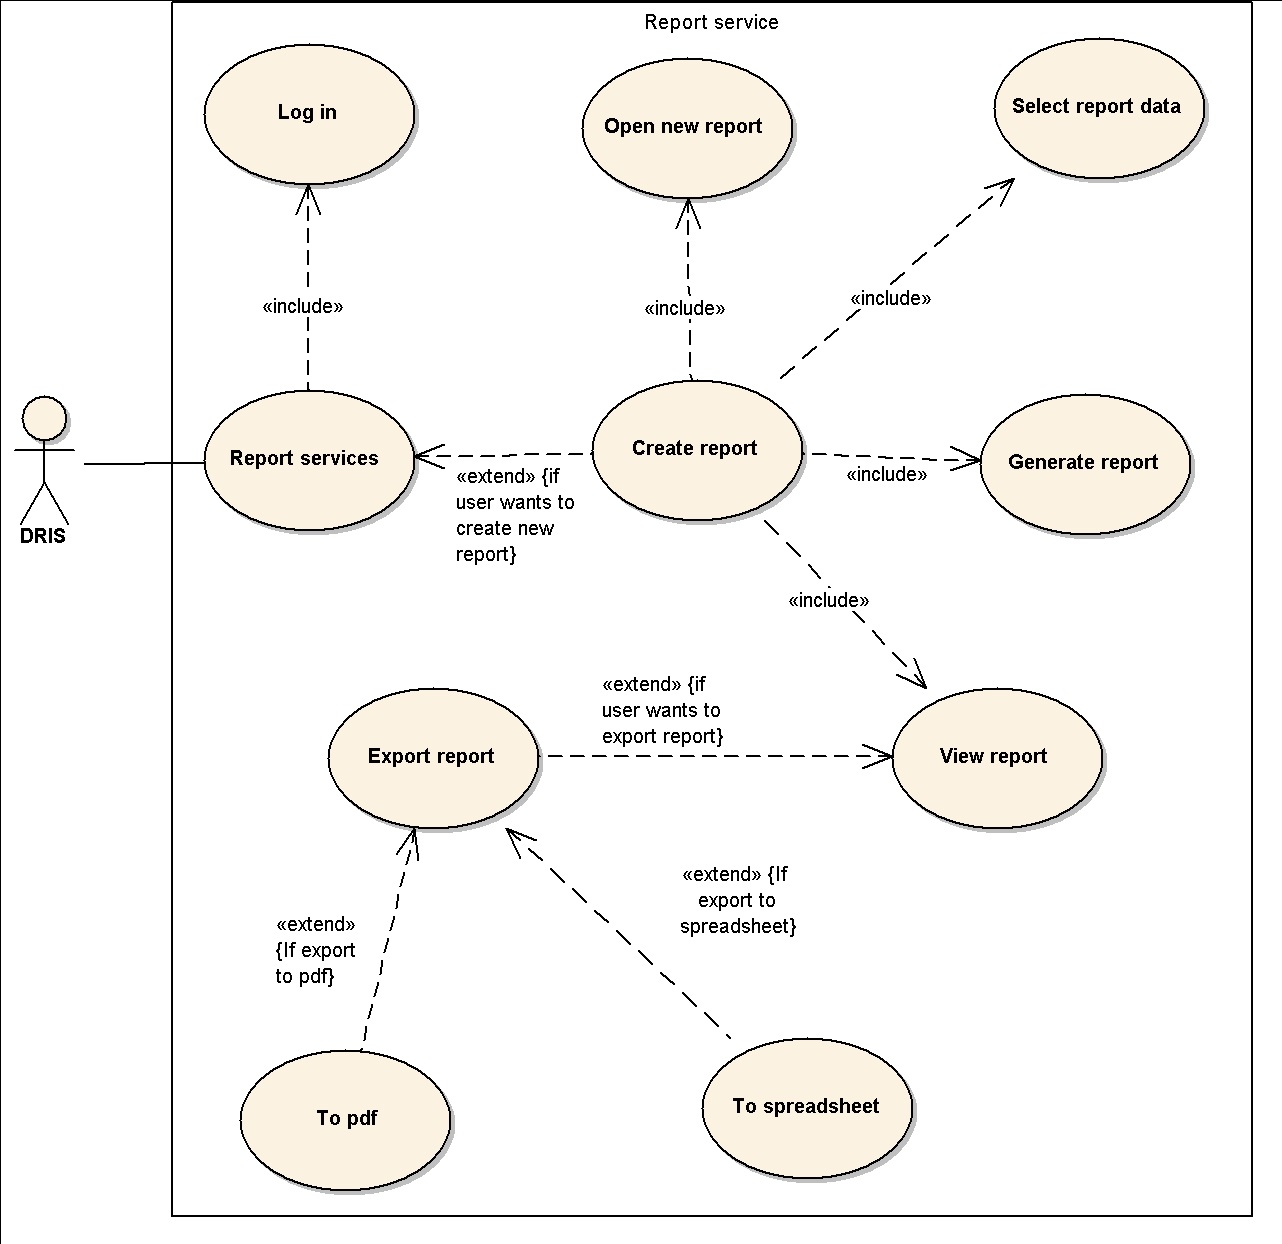
\includegraphics[scale=0.6]{../Images_Docs/Diagrams/Report service.jpg}}
\caption{Use case diagram of Report service}
\end{figure}

\begin{figure}[H]
\centering	
\framebox{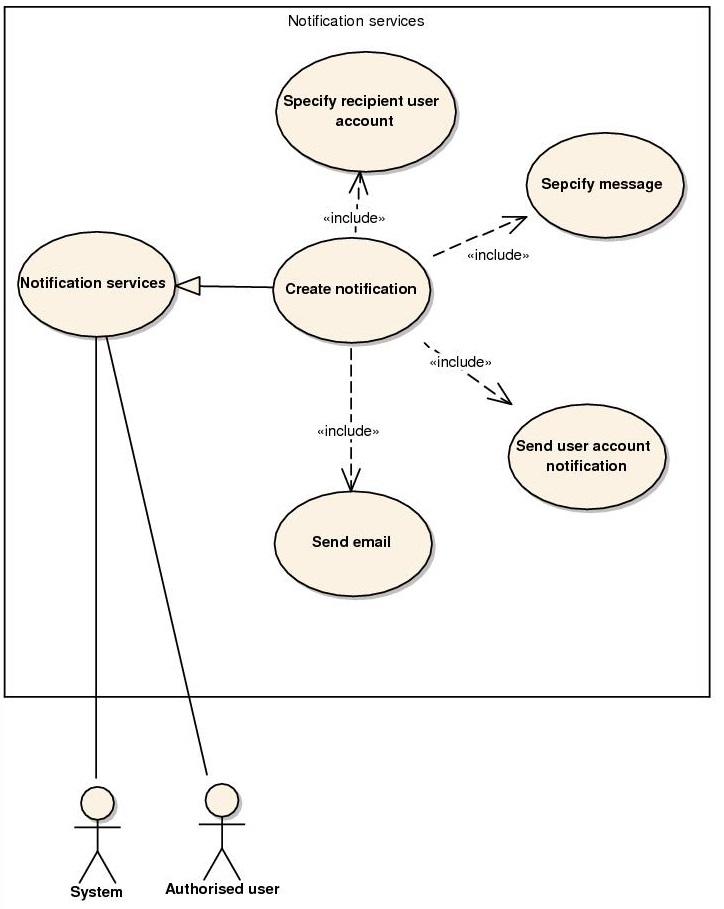
\includegraphics[scale=0.6]{../Images_Docs/Diagrams/Notification services.jpg}}
\caption{Use case diagram of Notification services}
\end{figure}

\begin{figure}[H]
\centering	
\framebox{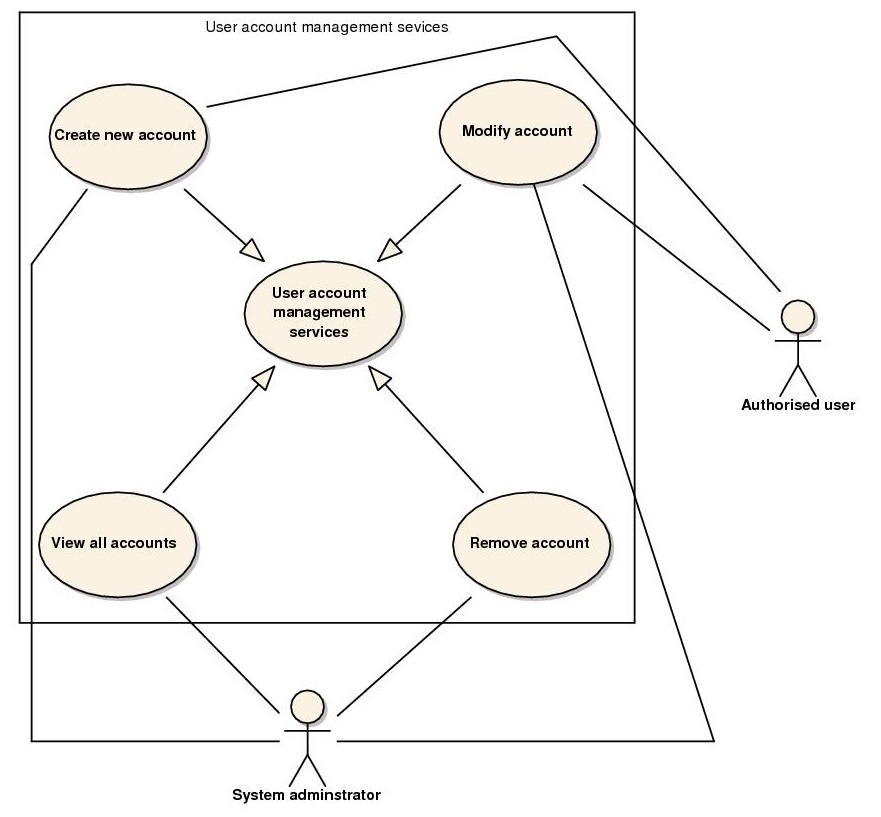
\includegraphics[scale=0.6]{../Images_Docs/Diagrams/User account management services.jpg}}
\caption{Use case diagram of User account management services}
\end{figure}

\begin{figure}[H]
\centering	
\framebox{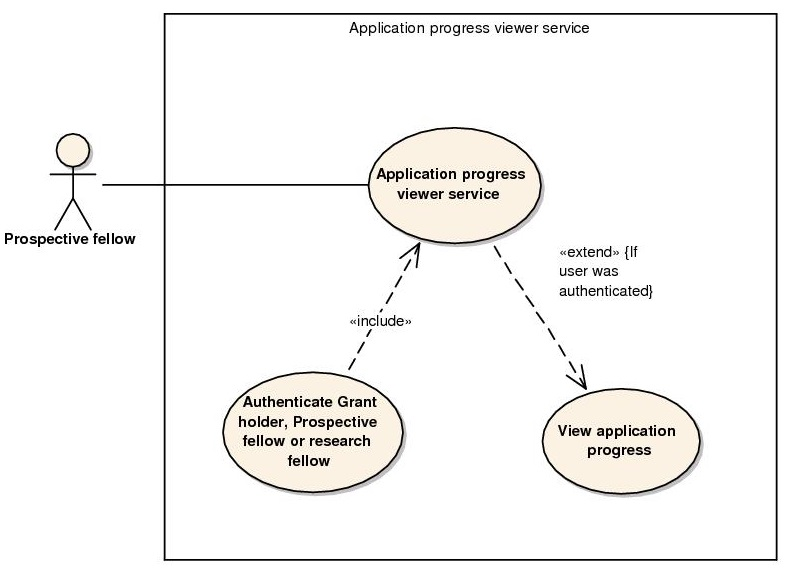
\includegraphics[scale=0.6]{../Images_Docs/Diagrams/Application/Application progress viewer service.jpg}}
\caption{Use case diagram of Application progress viewer service}
\end{figure}

\begin{figure}[H]
\centering	
\framebox{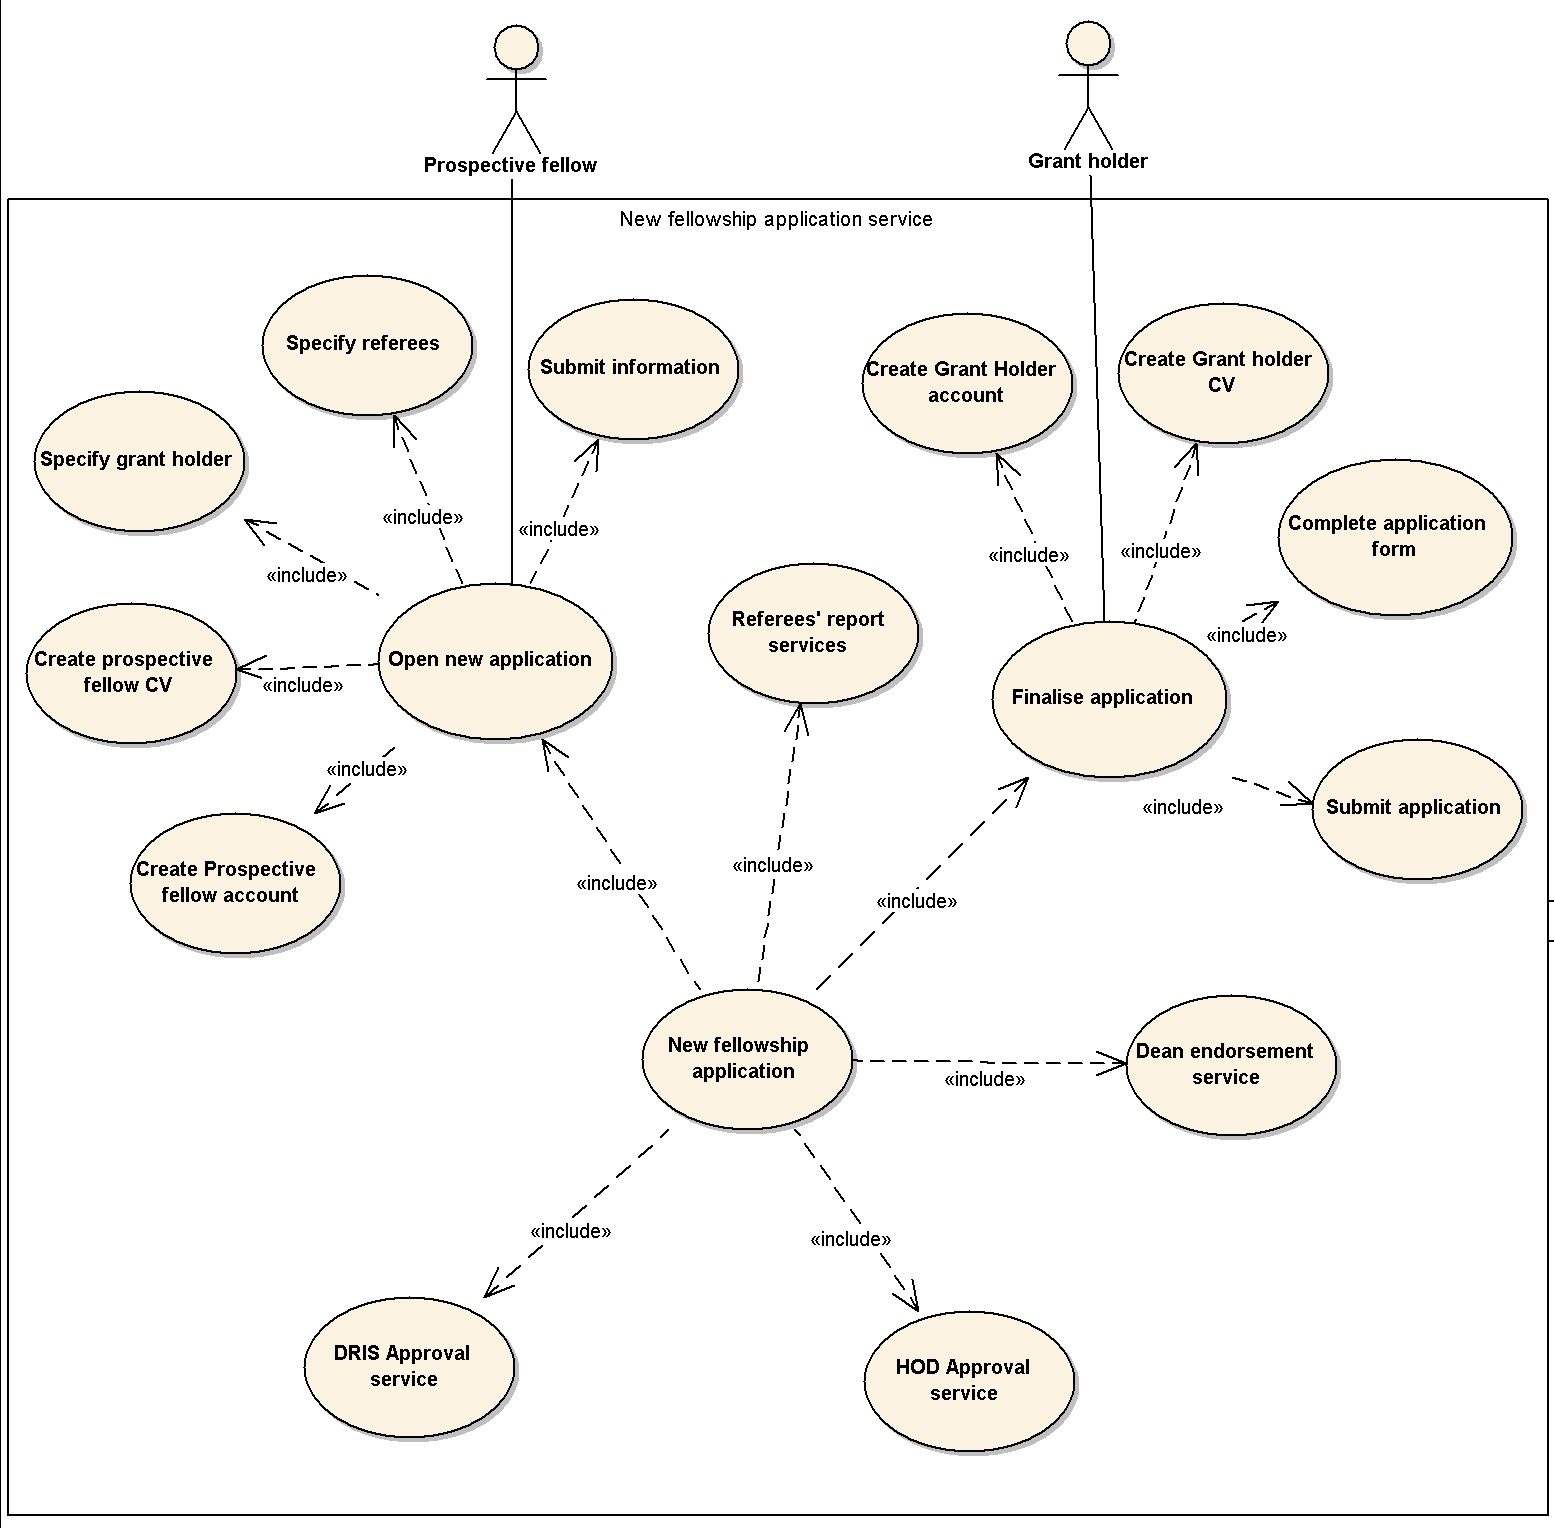
\includegraphics[scale=0.6]{../Images_Docs/Diagrams/Application/New fellowship application service.jpg}}
\caption{Use case diagram of New fellowship application service}
\end{figure}

\begin{figure}[H]
\centering	
\framebox{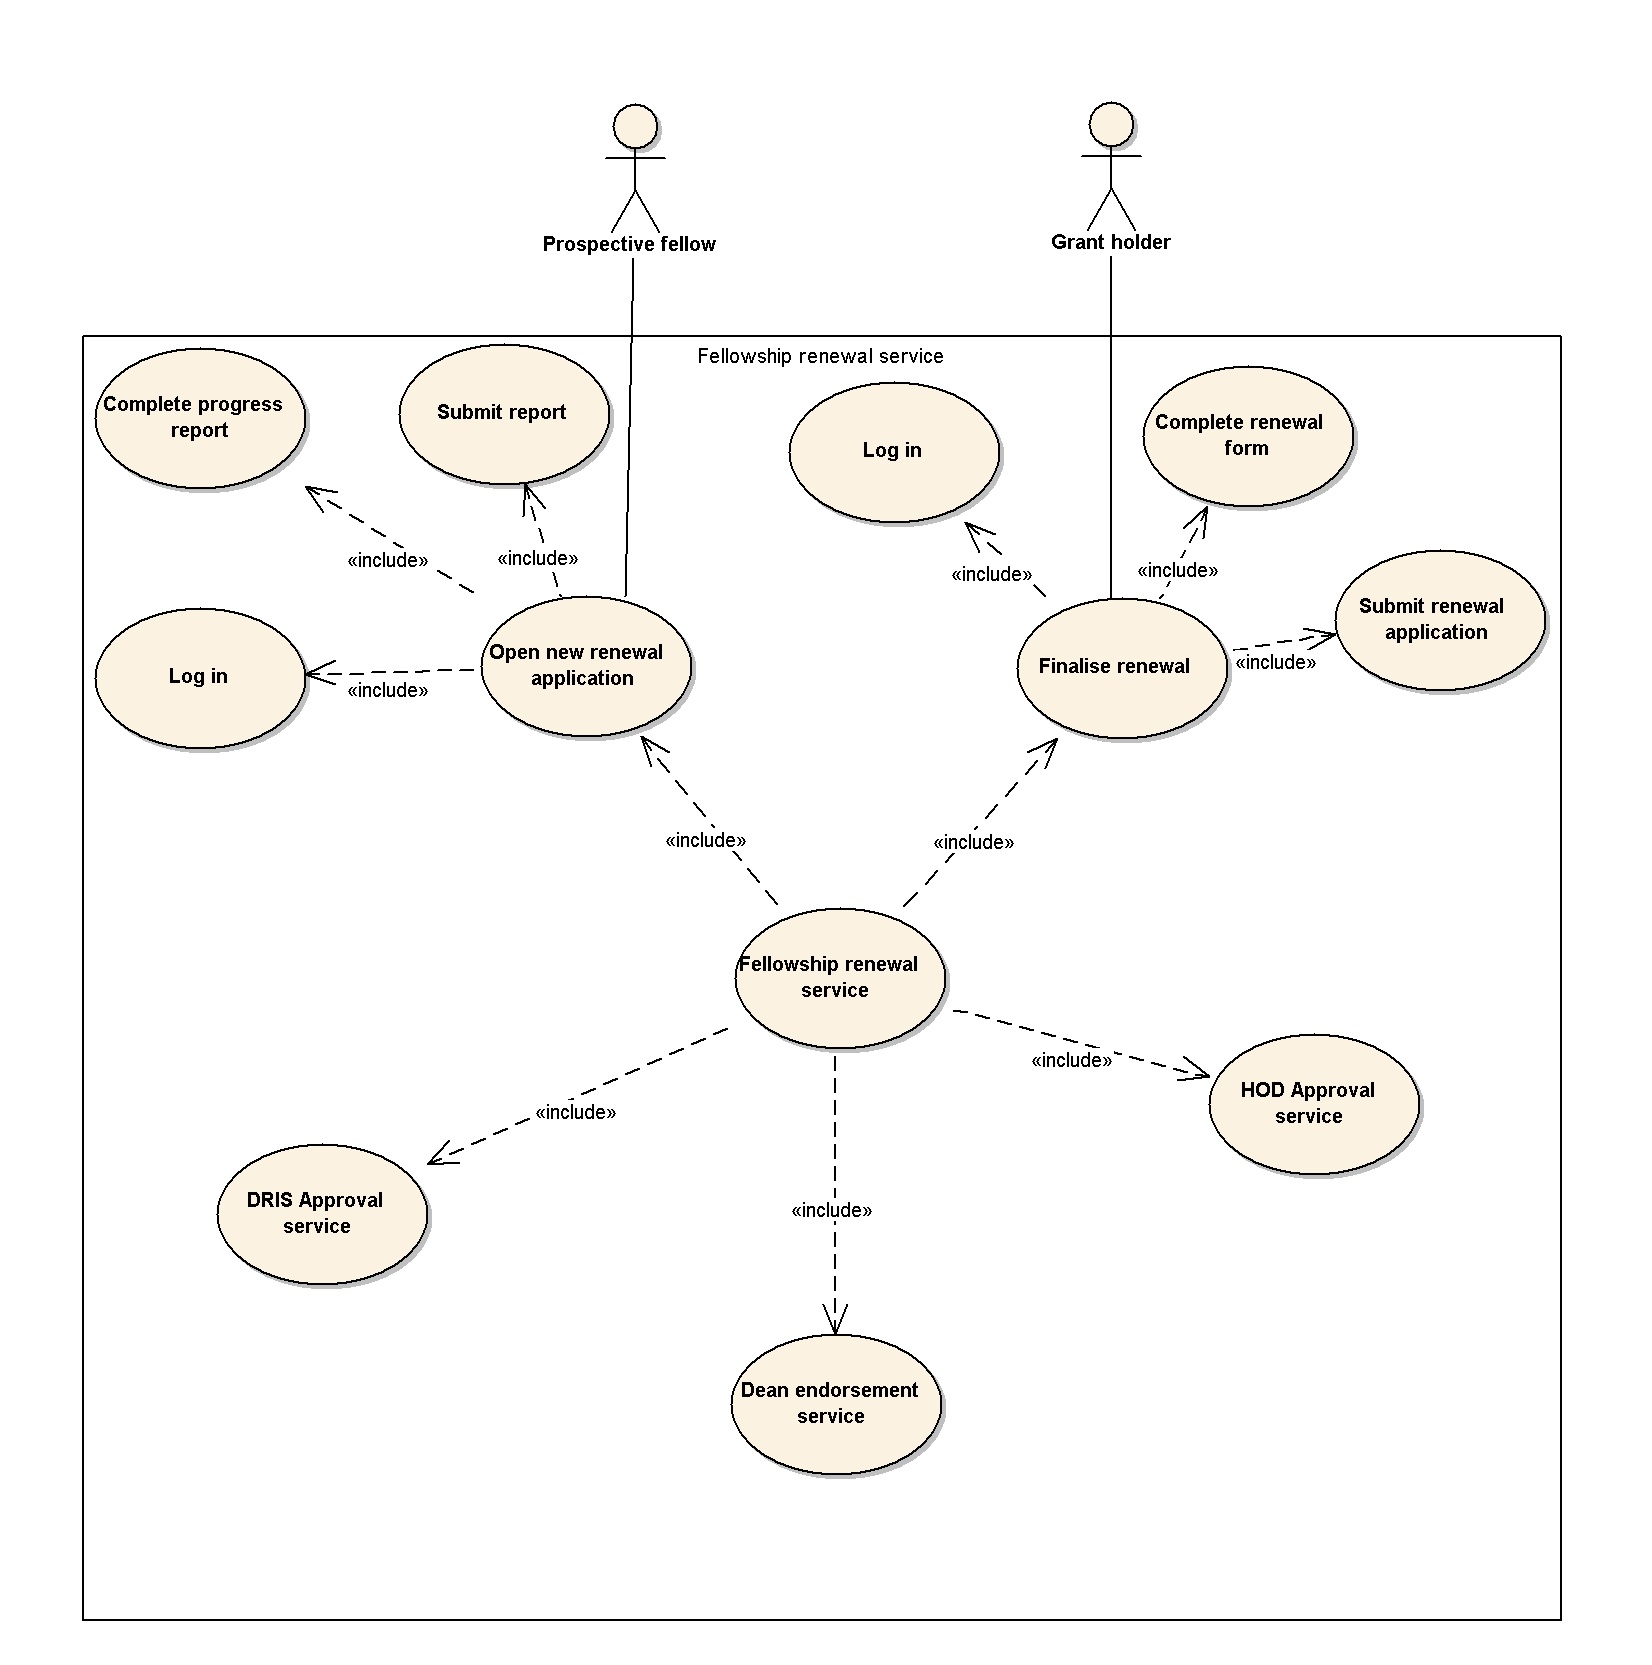
\includegraphics[scale=0.6]{../Images_Docs/Diagrams/Application/Fellowship renewal service.jpg}}
\caption{Use case diagram of Fellowship renewal service}
\end{figure}

\begin{figure}[H]
\centering	
\framebox{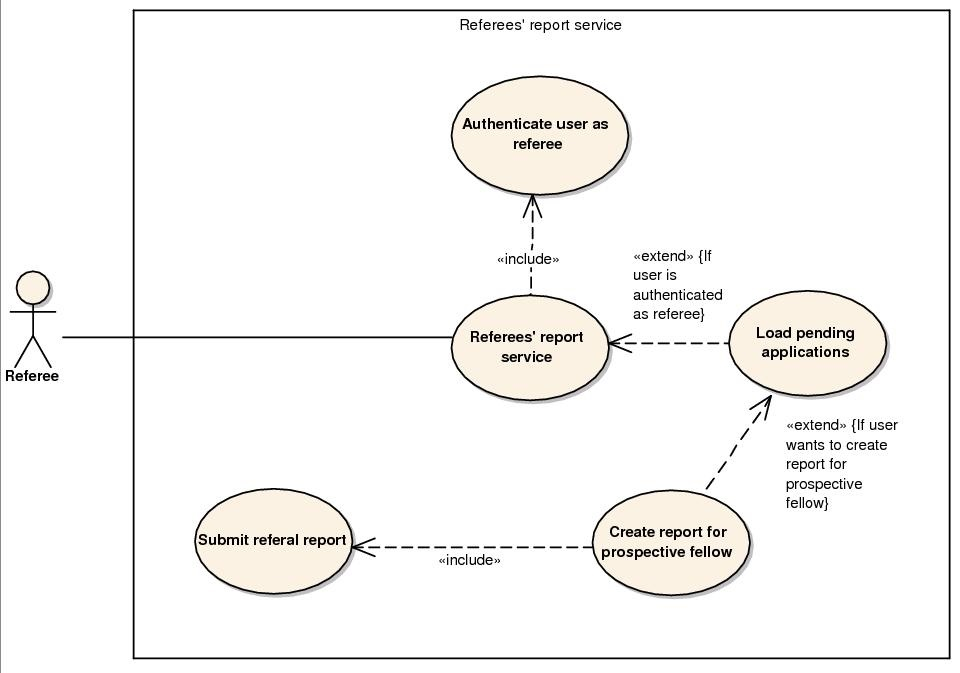
\includegraphics[scale=0.6]{../Images_Docs/Diagrams/Application/Referees' report service.jpg}}
\caption{Use case diagram of Referees' report service}
\end{figure}

\begin{figure}[H]
\centering	
\framebox{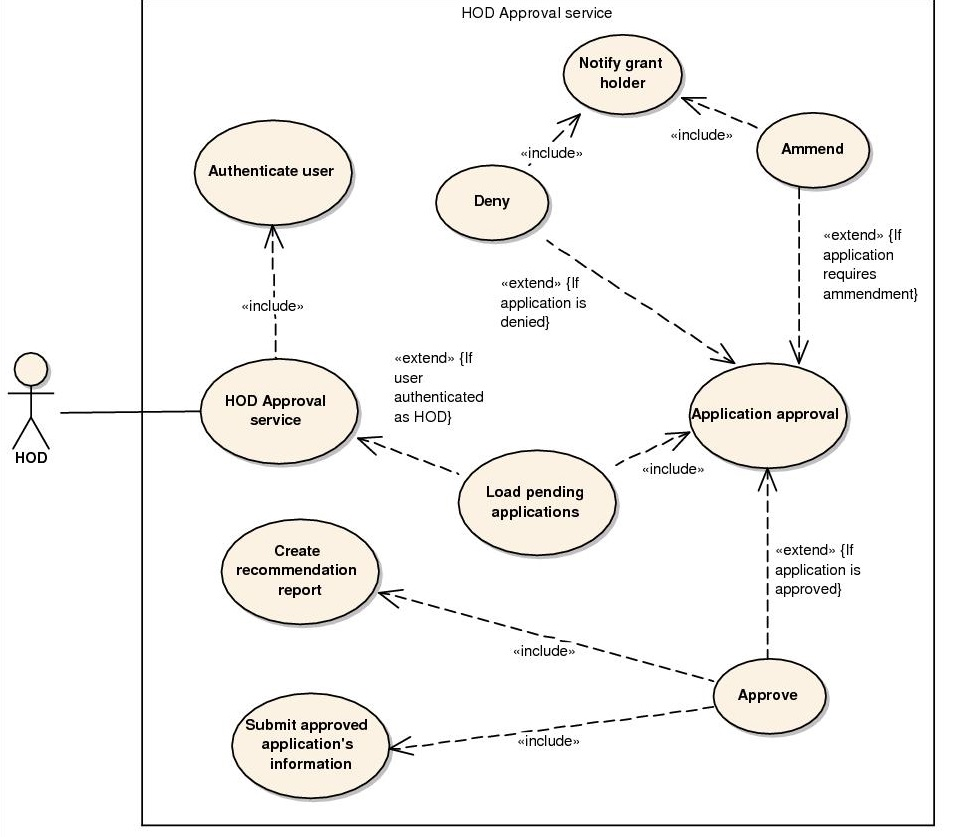
\includegraphics[scale=0.6]{../Images_Docs/Diagrams/Application/HOD Approval service.jpg}}
\caption{Use case diagram of HOD Approval service}
\end{figure}

\begin{figure}[H]
\centering	
\framebox{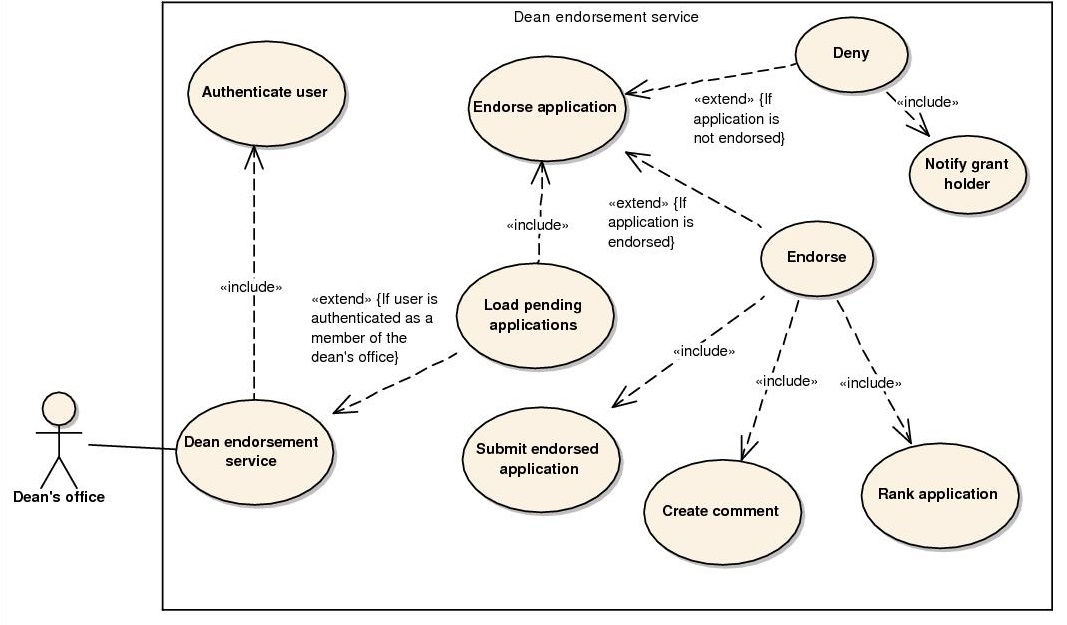
\includegraphics[scale=0.6]{../Images_Docs/Diagrams/Application/Dean endorsement service.jpg}}
\caption{Use case diagram of Dean endorsement service}
\end{figure}

\begin{figure}[H]
\centering	
\framebox{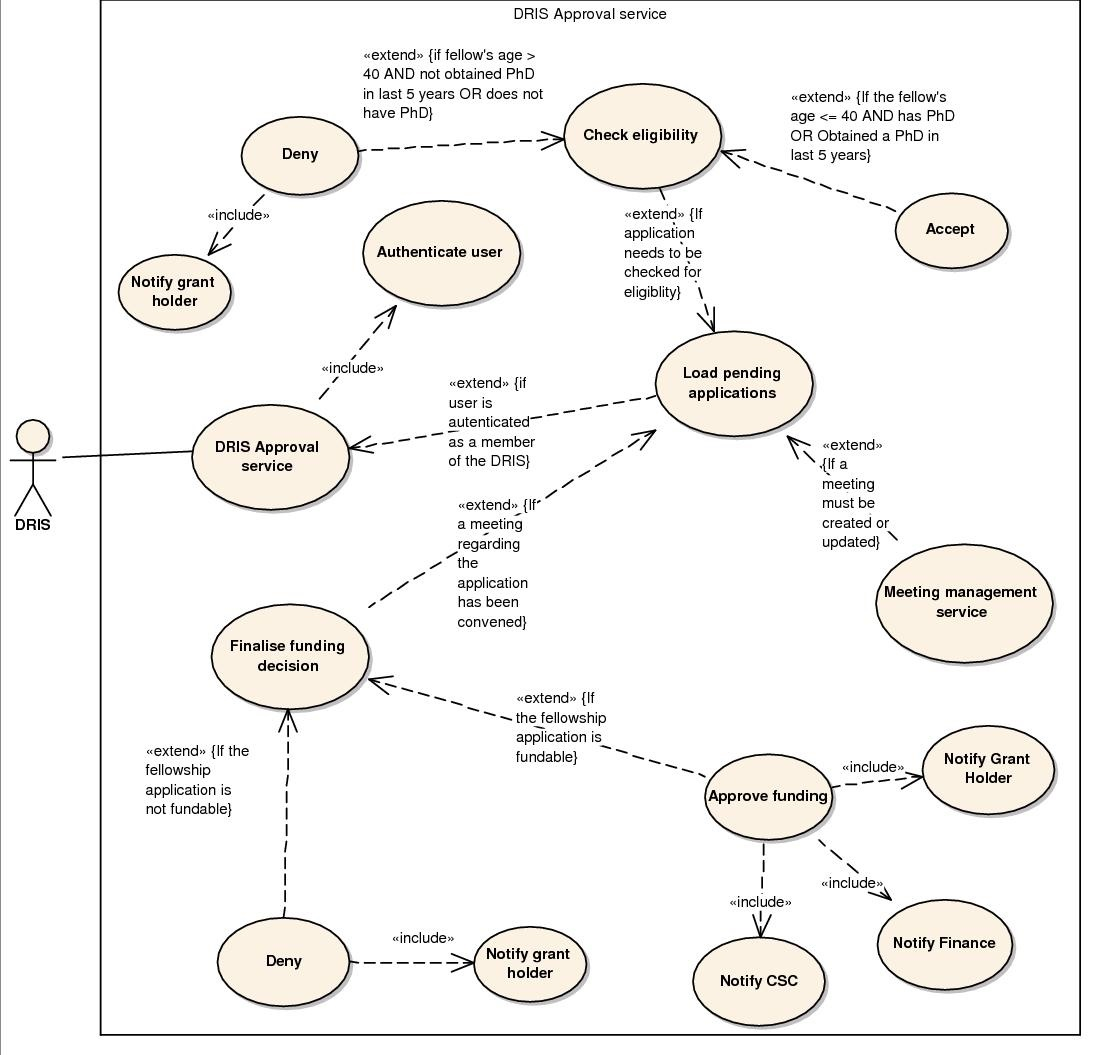
\includegraphics[scale=0.6]{../Images_Docs/Diagrams/Application/DRIS approval service.jpg}}
\caption{Use case diagram of DRIS approval service}
\end{figure}

\begin{figure}[H]
\centering	
\framebox{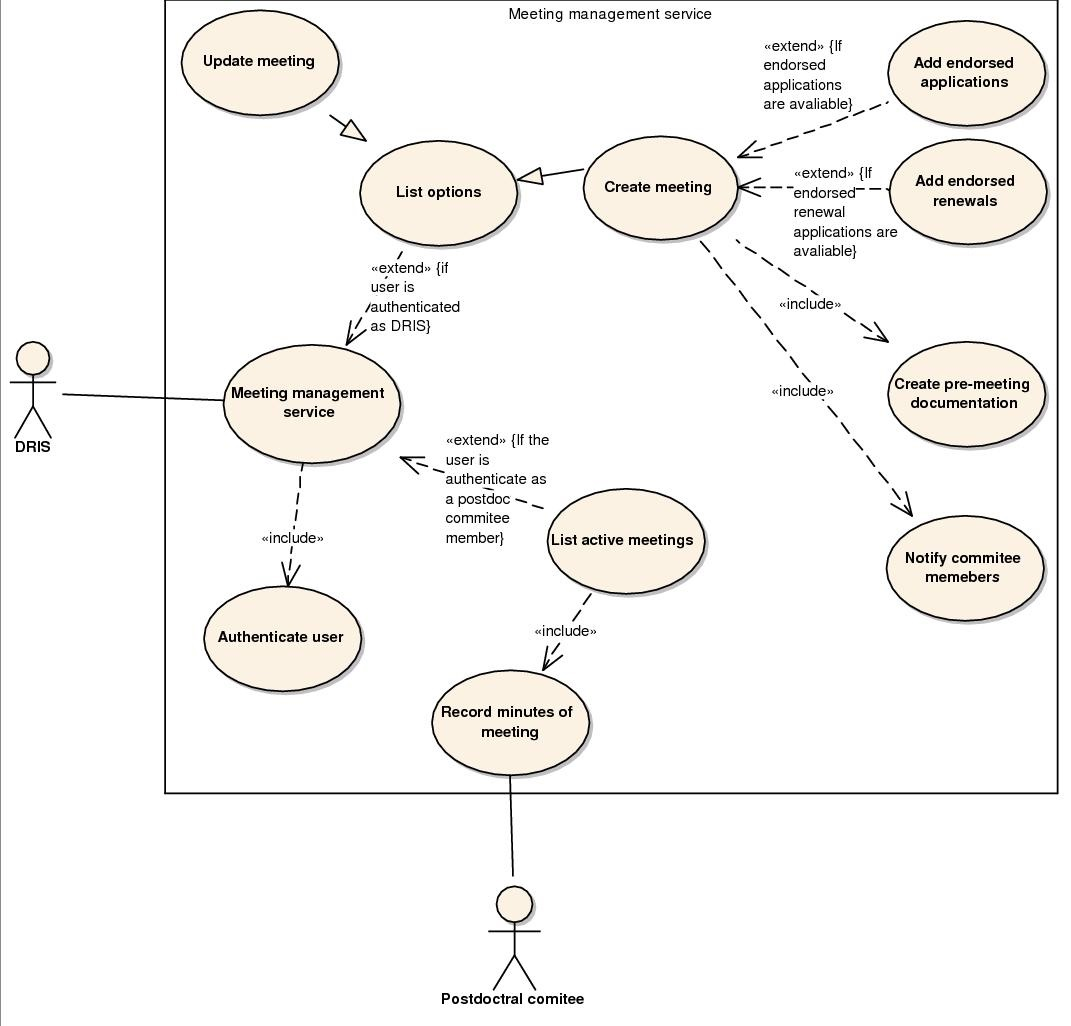
\includegraphics[scale=0.6]{../Images_Docs/Diagrams/Application/Meeting management service.jpg}}
\caption{Use case diagram of Meeting management service}
\end{figure}


\subsection{Use case prioritization} %Alfred
\vspace{0.2in}
This section states the ranking in terms of priority of the each use case per use case diagram figure. The priorities are: Critical, Important and Nice to have.\\ 
\begin{itemize}
	\item Application services: Critical
	\begin{itemize}
		\item New Application: Critical
		\item Renewal Application: Critical
		\item Application progress viewer service: Important
		\item Meeting management service: Nice To Have
	\end{itemize}
	\item Report services: Important
	\item Notification services: Critical
	\item User account management services: Critical
	\begin{itemize}
		\item Create new account: Critical
		\item Modify account: Critical
		\item Remove account: Critical
		\item Login: Critical
	\end{itemize}
	\item 
\end{itemize}


\vspace{0.2in}

\subsection{Use case/Services contracts} %Mathys
\vspace{0.2in}

This section states the preconditions and postconditions of the each use case per use case diagram figure. \\

\subsubsection{Preconditions}
These are conditions that must be met by the system or user before they are allowed to use the use case.\\
\begin{itemize}
	\item Fig 2.
	\begin{itemize}
		\item New fellowship application service: Can only be accessed if new applications are open.
		\item Fellowship renewal service: Can only be accessed if renewals are open.
		\item Application progress viewer service: Can only be accessed if user logged in with correct security permissions.	
	\end{itemize}
	
	\item Fig 3.
		\begin{itemize}
			\item Log in: If a user with the associated credentials has appropriate security role.
			\item Create report: If user is logged in.
			\item Open new report: If no report is currently open.
			\item Select report data: If report is open and data is available for report.
			\item Generate report: If data has been selected.
			\item View report: If a report has been generated.
			\item Export report: If user wants to export report.
			\item To spreadsheet: If user wants to export report to a spreadsheet.
			\item To pdf: If user wants to export report to a pdf.	
		\end{itemize}
	
	\item Fig 4.
			\begin{itemize}
				\item Create notification: If requesting user is the system.
				\item Specify recipient user account: If a notification is in its setup stage.				
				\item Specify message: If a notification is in its setup stage.
				\item Send user account notification: If notification is ready to be sent.
				\item Send email: If notification is ready to be sent.	
			\end{itemize}
	
	\item Fig 5.
			\begin{itemize}
				\item Create new account: If requesting user has the appropriate security role.
				\item Modify account: If requesting user has the appropriate security role or is the owner of the account.				
				\item Remove account: If requesting user has the appropriate security role.						
			\end{itemize}
	
	\item Fig 6.
		\begin{itemize}
			\item View application progress: Can only be used if there are any applications made by the user.
		\end{itemize}
		
	\item Fig 7.
		\begin{itemize}
			\item Create prospective fellow account: If prospective fellow does not have an account.
			\item Submit information: If all the application information is complete.				
			\item Create grant holder account: If grant holder does not have an account.
			\item Create grant holder cv: If the grant holder does not have an NRF rating or does have never created a CV on the system before.
			\item Submit application: If all the required information has been entered.									
		\end{itemize}
	
	\item Fig 8.
		\begin{itemize}
			\item Open new renewal application: If prospective fellow has a fellowship that is renewable.
			\item Submit report: If progress report is completed.				
			\item Submit renewal application: If all the required information for the renewal has been entered.									
		\end{itemize}
	
	\item Fig 9.
		\begin{itemize}
			\item Create referee account: If the referee does not have an account.
			\item Create report: If requesting user has the appropriate security role.				
			\item Submit referral report: If the referral report has been completed.									
		\end{itemize}
		
	\item Fig 10.
		\begin{itemize}
			\item Application approval: If any finalised application is available for approval and the grant holder of the application falls under department the HOD is in charge of.
			\item Create recommendation report: If the application has been approved.				
			\item Submit approved application's information: If the recommendation report has been completed.									
		\end{itemize}
		
	\item Fig 11.
		\begin{itemize}
			\item Endorse application: If any approved application is available for endorsement and the grant holder of the application falls under faculty of which the Dean's office is in charge of.
			\item Rank application: If the application has been endorsed.	
			\item Create comment: If the application has been ranked.			
			\item Submit endorsed application: If the required endorsement information has been completed.									
		\end{itemize}
	
	\item Fig 12.
		\begin{itemize}
			\item Check eligibility: If any endorsed application is available for its eligibility check.
			\item Deny: If the prospective fellow is older than 40 and has not obtained their PhD in the last 5 years or if the prospective fellow does not have a PhD.
			\item Accept: If the prospective fellow is younger than 40 or is 40 and they have a PhD or if they have obtained a PhD in the last 5 years. 
			\item Finalise funding decision: If the meeting regarding the application has been concluded.	
			\item Deny: If the application's funding was denied.			
			\item Approve funding: If the application's funding was denied.									
		\end{itemize}
	
	\item Fig 13.
		\begin{itemize}
			\item Create meeting: If any eligible applications are available.
			\item Add endorsed applications: If any new applications that are eligible are available.
			\item Add endorsed renewals: If any renewal applications that are eligible are available.
			\item Record minutes of meeting: If the selected meeting has been setup.							
		\end{itemize}
	\end{itemize}

\subsubsection{Postconditions}
These are conditions that must be met by the system and the data after the use case has been used.\\
\begin{itemize}
		
	\item Fig 3.
		\begin{itemize}
			\item Log in: The user has been authenticated and has the appropriate security role.
			\item Open new report: A new report is active.
			\item Select report data: The data for the active report is selected.
			\item Generate report: The report is available for viewing.
			\item View report: The report is available for export and must be visible.	
		\end{itemize}
	
	\item Fig 4.
			\begin{itemize}
				\item Create notification: A possible notification is open for receiving its contents.
				\item Specify recipient user account: The notification has a a recipient.				
				\item Specify message: The notification has a message.
				\item Send user account notification: The message is sent to the user.
				\item Send email: The message is sent the email associated with recipients user account.	
			\end{itemize}
	
	\item Fig 5.
			\begin{itemize}
				\item Create new account: A new user account is added to the system.
				\item Modify account: The specified user account is updated.				
				\item Remove account: The specified user account is removed from the system.						
			\end{itemize}
	
	\item Fig 6.
		\begin{itemize}
			\item View application progress: The application progress of the specified user application is visible.
		\end{itemize}
		
	\item Fig 7.
		\begin{itemize}
			\item Create prospective fellow account: If prospective fellow has an account.
			\item Create prospective fellow cv: The CV is created and associated with the prospective fellow and the application.
			\item Specify grant holder: The grant holder's contact information is associated with the application.
			\item Specify referees: The referees' contact information is associated with the application.
			\item Submit information: The initial application data is complete. Referees are notified.				
			\item Create grant holder account: The grant holder has an account.
			\item Create grant holder cv: The grant holder's CV is associated with the application.
			\item Complete application form: The application data is complete and the application is ready to be finalised.
			\item Submit application: The application is now a finalised application and the HOD of the relative department is notified. 									
		\end{itemize}
	
	\item Fig 8.
		\begin{itemize}
			\item Open new renewal application: A new renewal is for a fellowship is open.
			\item Log in: The user has been authenticated and has the appropriate security role.
			\item Complete progress report: The progress report associated with	the renewal.		
			\item Submit report: The initial renewal information is complete. Grant holder is notified.
			\item Complete renewal form: The renewal data complete and the renewal is ready to be finalised.			
			\item Submit renewal application: The renewal application is finalised and the HOD of the relative department is notified.									
		\end{itemize}
	
	\item Fig 9.
		\begin{itemize}
			\item Create referee account: Referee has a user account.
			\item Log in: The user has been authenticated and has the appropriate security role.
			\item Create report: The report is complete and ready to be submitted.				
			\item Submit referral report: The referral report has been finalised and associated with the application and the Grant Holder of the application is notified.									
		\end{itemize}
		
	\item Fig 10.
		\begin{itemize}
			\item Log in: The user has been authenticated and has the appropriate security role.
			\item Deny: Application has status changed to denied.
			\item Amend: Application is reopened and status changed to amend.
			\item Notify grant holder: A notification is sent to the Grant holder of the application.  
			\item Approve:  The application recommendation report becomes available for completion.
			\item Create recommendation report: The recommendation report is associated with the application and the Approval is ready to be finalised.				
			\item Submit approved application's information: The application approval is finalised and the application is now a approved application and the Dean's Office of the relevant faculty is notified.									
		\end{itemize}
		
	\item Fig 11.
		\begin{itemize}
			\item Log in: The user has been authenticated and has the appropriate security role.
			\item Deny: The application's status is changed to denied. 
			\item Notify grant holder: A notification is sent to the Grant holder of the application.
			\item Endorse: The application's endorsement information becomes available for completion.
			\item Rank application: The application has a rank associated with it.	
			\item Create comment: The application has a endorsement comment associated with it.			
			\item Submit endorsed application: The application endorsement is finalised and the application is now an endorsed application and the DRIS is notified.									
		\end{itemize}
	
	\item Fig 12.
		\begin{itemize}
			\item Log in: The user has been authenticated and has the appropriate security role.
			\item Deny: The application's status is changed to denied. 
			\item Notify grant holder: A notification is sent to the Grant holder of the application.
			\item Accept: The application is ready for discussion and is now an eligible application.			
			\item Deny: The application's status is changed to denied.			
			\item Approve funding: The application is now a complete application.
			\item Notify grant holder: A notification is sent to the Grant holder of the application.
			\item Notify CSC: A notification is sent to the CSC.
			\item Notify Finance: A notification is sent to the Finance department.									
		\end{itemize}
	
	\item Fig 13.
		\begin{itemize}
			\item Create meeting: A new meeting is open for modification.
			\item Add endorsed applications: An endorsed new application has been added to the agenda of the meeting.
			\item Add endorsed renewals: An renewal application has been added to the agenda of the meeting.
			\item Create pre-meeting documentation: Documentation complete and associated with meeting and the meeting is closed for modification.
			\item Notify committee members: A notification is sent to all the committee members.
			\item Record minutes of meeting: The meeting is finalised and it's minutes stored.							
		\end{itemize}

\end{itemize}


\vspace{0.2in}

%\subsection{Process specifications} %Alfred
%\vspace{0.2in}

%\vspace{0.2in}

\subsection{Domain Objects} %Alfred
\subsubsection{Overview}

\begin{figure}[H]
\centering	
\framebox{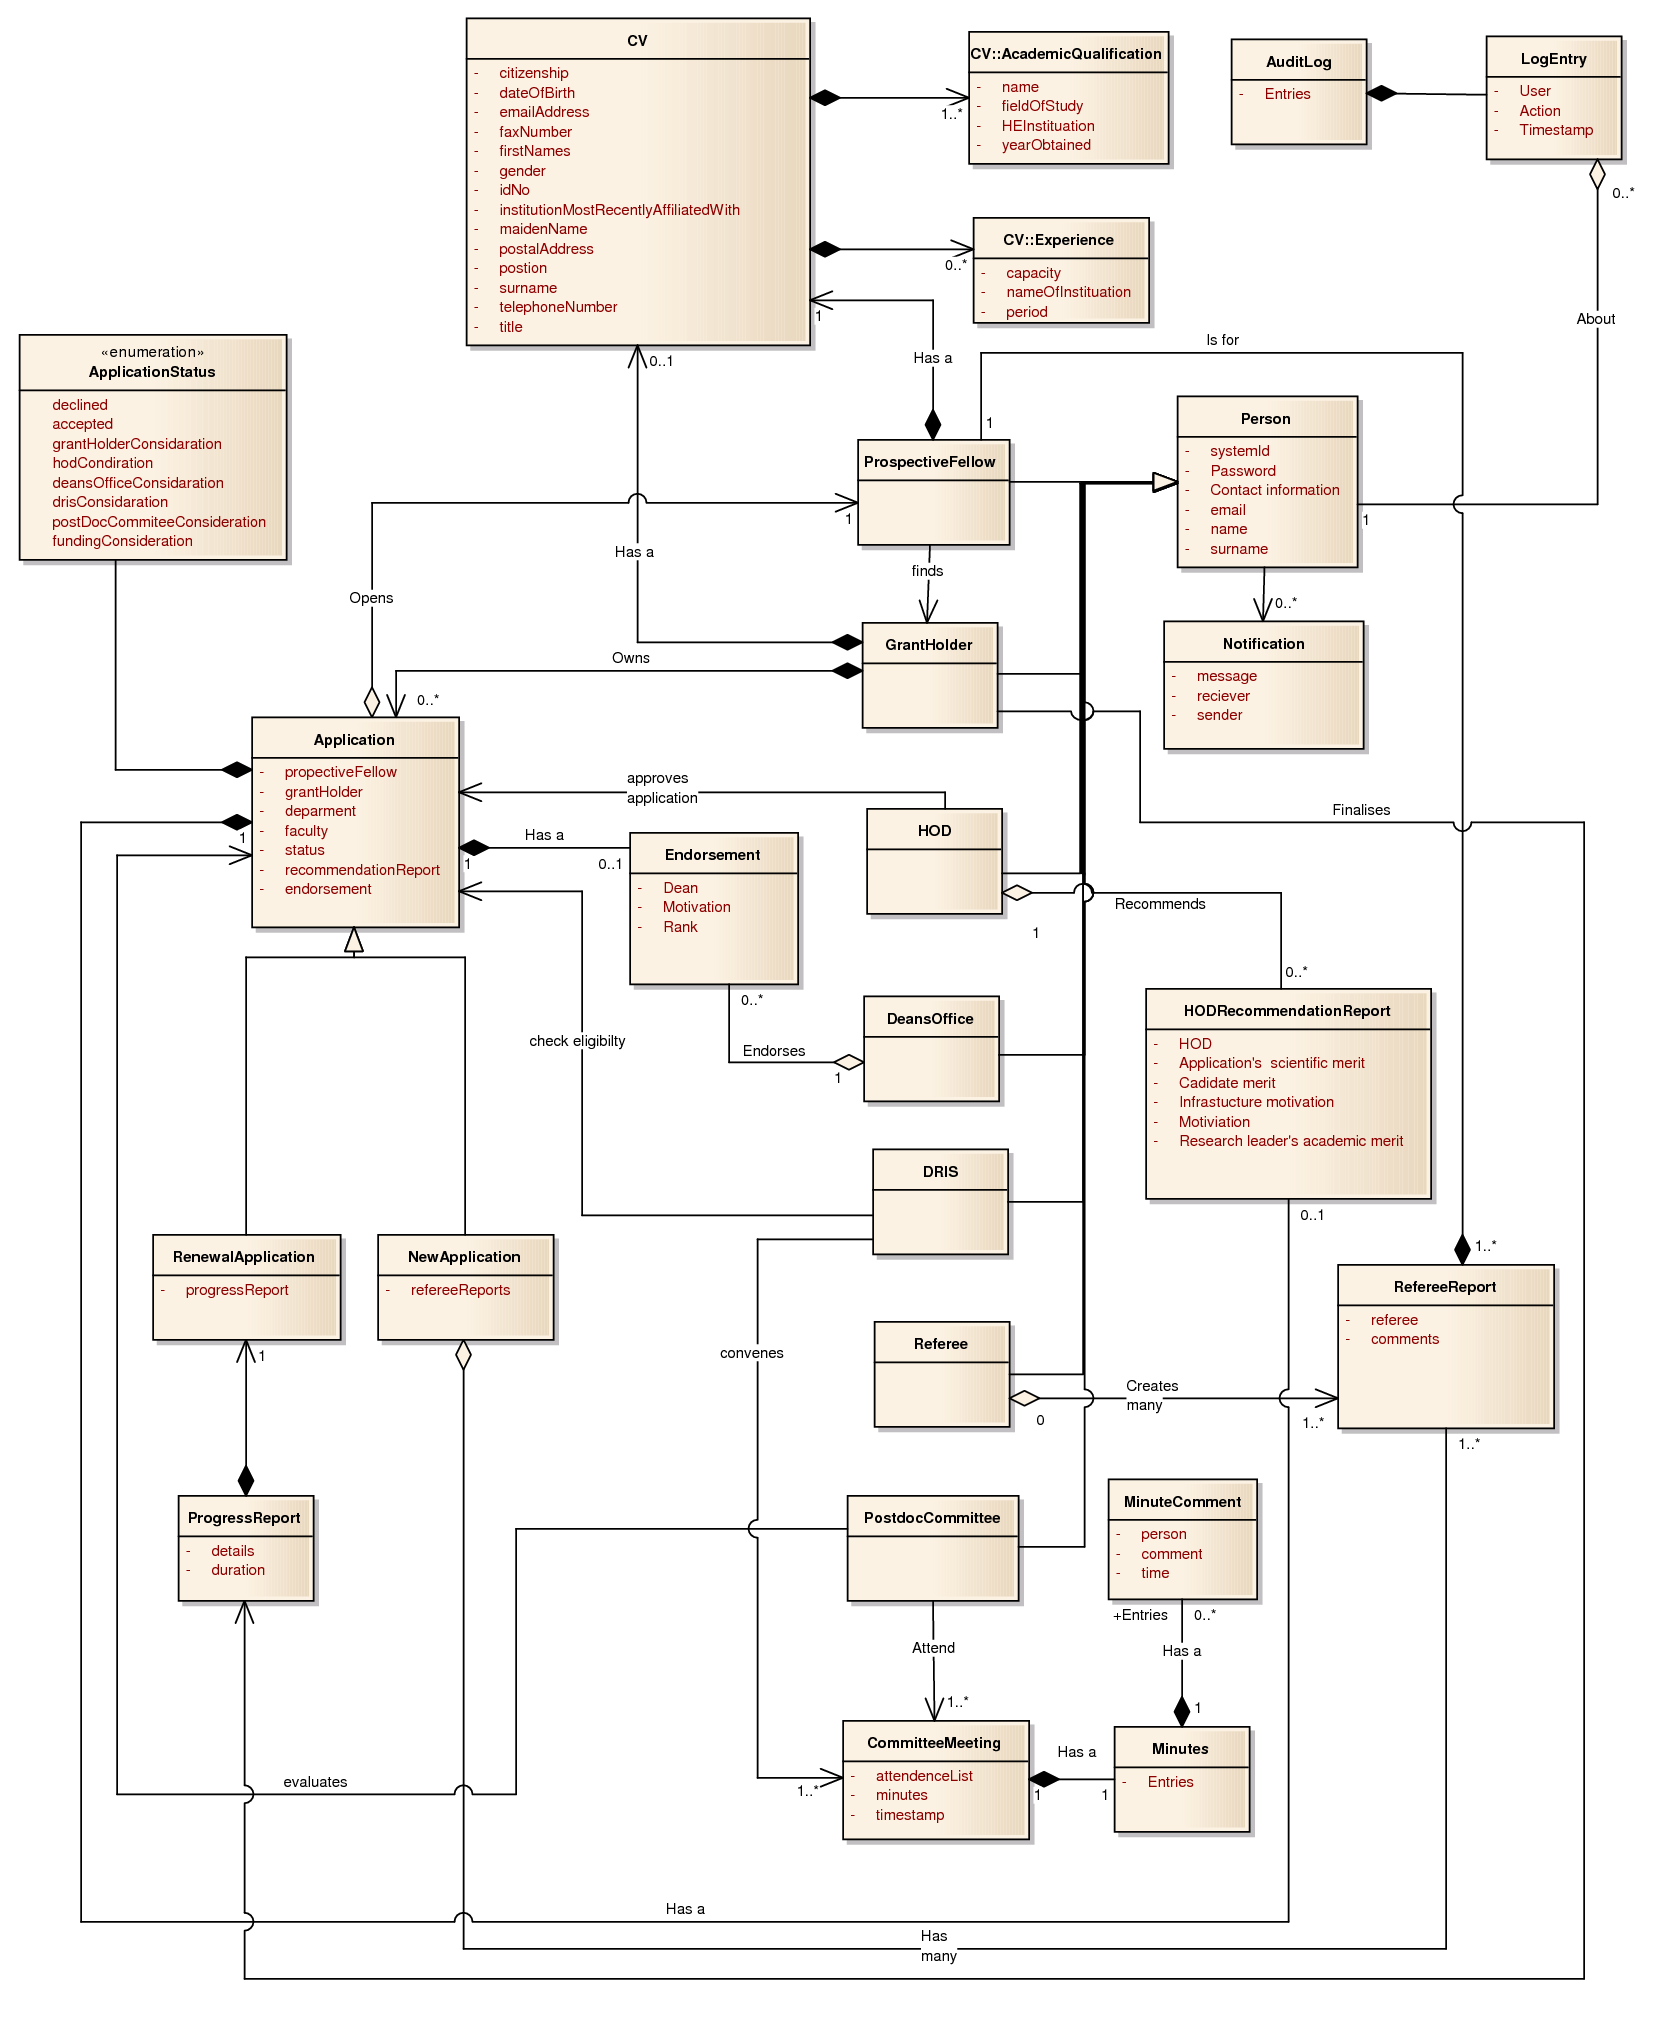
\includegraphics[scale=0.55]{../Images_Docs/Diagrams/DomainObjects/DomainObjects.png}}
\caption{Overview of the data structures and relationships for the core domain objects of the
system.}
\end{figure}

\newpage
\subsubsection{Persons}
This object represents the stakeholders that will make use of the system. All stakeholders will have accounts which they will use to log on to the system. Using a unique user id and a predefined or user specified password. The unique user id can either be a Peoplesoft Emplid number or a email address.

\subsubsection{DRIS}
This object represents members of Department of Research and Innovation Support who administers the process.

\subsubsection{ProspectiveFellow}
This object represents a prospective fellow who is a holder of a PhD obtained in the last five years (or nearing completion of a PhD) or is 40 years or younger and has a PhD.

\subsubsection{GrantHolder}
This object represents a grant holder who can be a rated researcher by the NRF or not. The system should not require the CV's of A and B rated researchers to be added to the system. The reason for this is that the CV's of such researchers can be easily obtained from the NRF and tend to be very long. A grant holder is the supervisor for a or many \textbf{ProspectiveFellow}(s) and owns the \textbf{Application} of the \textbf{ProspectiveFellow}(s).

\subsubsection{HOD}
This object represents a HOD of a particular department. The HOD creates the recommendation reports for \textbf{Application}(s) they consider to meet their requirements.\\

\subsubsection{HODRecommandationReport}
This object represents a recommendation report highlighting the reasons to why the \textbf{Application} of a \textbf{ProspectiveFellow} is needed by the department.

\subsubsection{Deans Office}
The Dean's office object represents the relevant faculty's Dean and Deputy Dean. The Dean's Office creates the \textbf{Endorsement} for any the \textbf{Application} that is approved by them.

\subsubsection{Endorsement}
This object represents the endorsement of an \textbf{Application} of a \textbf{ProspectiveFellow} and contains the rank in comparison to other pending \textbf{Application}(s).

\subsubsection{Referee}
This object represents the referees of any \textbf{ProspectiveFellow} and is responsible for creating \textbf{RefereeReport} regarding the \textbf{ProspectiveFellow}.

\subsubsection{RefereeReport}
This object represents the referral report from an identified referee of a \textbf{ProspectiveFellow}.

\subsubsection{PostDocCommittee}
This object represents the individual members of the post-doctoral committee who approves all available \textbf{Applications} during committee meetings and records the \textbf{Minutes} of the meeting.

\subsubsection{CommitteeMeeting}
This object represents a meeting of the \textbf{PostDocCommittee} convened by the \textbf{DRIS} that will be review the \textbf{Applications} and will evaluate each. This object contains the attendance list, date and time convened and the \textbf{Minutes} of the meeting.

\subsubsection{Minutes}
This object represents the minutes of the \textbf{CommitteeMeeting} and holds the multiple \textbf{MinuteComment}(s) of the meeting.

\subsubsection{MinuteComment}
This object represents a comment made by a \textbf{PostDocCommittee} member during a \textbf{CommitteeMeeting}.

\subsubsection{Application}
This object represents an applications and will contain the information of \textbf{ProspectiveFellow} and \textbf{GrantHolder} who owns it. The object holds the status of the application. As well as the \textbf{HODRecommandationReport} of a \textbf{HOD} and \textbf{Endorsement} from a \textbf{DeansOffice}.

\subsubsection{NewApplication}
This inherited object represents new application for a \textbf{ProspectiveFellow} who is currently not a fellow in the system. Also it holds any \textbf{RefereeReport}(s) that has been created for the application.

\subsubsection{RenewalApplication}
This inherited object represents renewal application for a \textbf{ProspectiveFellow} who is a fellow in the system. Also it holds the \textbf{ProgressReport} that has been created for the application.

\subsubsection{ProgressReport}
This object represents a report on the research that the \textbf{ProspectiveFellow} had done through the duration of their fellowship.

\subsubsection{CV}
This object represents a CV and contains all the information such as personal details, \textbf{AcademicQualification}(s), \textbf{Experience} regarding a \textbf{GrantHolder} or \textbf{ProspectiveFellow} in the system.

\subsubsection{AcademicQualification}
This object represents a academic qualification and the information regarding it such as the qualification name, field, where it was obtained and when it was obtained.

\subsubsection{Experience}
This object represents a work experience and the information regarding it such as the capacity of the work, where this work was done and when it was done.

\subsubsection{Notification}
This object represents a email or internal message sent by a user to a user via the system. The system itself may also seen as a user in this regard.

\subsubsection{AuditLog}
This object represents a audit log that stores all the actions of all users within the system.

\subsubsection{LogEntry}
This object represents a \textbf{AuditLog} entry which records the action, who committed the action as well as at what time the action was committed.



\newpage	

\newpage
\section{Glossary:}
\vspace{0.2in}

\begin{itemize}

\item \textbf{API} - Application Programming Interface
\item \textbf{Application} -Both renewal applications or new fellowship applications are seen as applications by this project.
\item \textbf{CV} - Curriculum Vita
\item \textbf{HTML} - Hyper Text Mark-up Language
\item \textbf{Java EE} - Java Enterprise Edition
\item \textbf{NRF} - National Research Foundation
\item \textbf{PhD} - A doctoral degree in a particular field of study.
\item \textbf{PDF} - Portable Document Format file
\item \textbf{Spreadsheet} - A special type of digital document that is used to represent data in rows and columns
\item \textbf{Use case} - A visual depiction of a service or group of services.
\item \textbf{UML} - Unified modelling language. A commonly used model standard to provide technology neutral models of different aspects of software.
\item \textbf{UP} - University of Pretoria
 


\end{itemize}	

\end{document}